\chapter{Драйвер I2C устройства}
\textbf{Цель:} Активировать I2C контроллер, и написать простой драйвер для устройства подключённого к I2C шине.

\vspace{5mm}
\textbf{Описание:}Работа с I2C интерфейсом не требует разработки модуля ядра, при условии, что внешний модуль не требует дополнительных управляющих линий. В ОС Linux есть набор программных продуктов, позволяющих сканировать (i2cdetect) подключённые модули, с целью определения адресов устройств на шине, а так же для контроля исправности. Так же модули позволяющие отправлять (i2c\_set) и принимать (i2c\_get) данные .

В данной работе, будет приведён пример приложения, обеспечивающего настройку и взаимодействие с внешним модулем GY-87 предсталяющем собой навигационный модуль с 10-ю степенями свободы (3-х осевой гироскоп и 3-х осевой акселерометр MPU6050, 3-х осевой датчик магнитного поля HMC5883L и барометр BMP180). 

\vspace{5mm}
\textbf{Полезные ссылки:}
\begin{itemize}
	\item \href{http://www.gaw.ru/html.cgi/txt/interface/iic/start.htm}{Последовательный интерфейс I2C}.
	\item \href{https://docs.kernel.org/devicetree/dynamic-resolution-notes.html}{Kernel Doc: Devicetree Dynamic Resolver Notes}
	\item \href{https://www.kernel.org/doc/html/v4.15/driver-api/i2c.html}{Kernel Doc: I2C API}	
	\item \href{https://hadex.cz/spec/m442d.pdf}{описание модуля GY-87}
	\item \href{https://invensense.tdk.com/wp-content/uploads/2015/02/MPU-6000-Datasheet1.pdf}{TDK MPU6050: описание}
	\item \href{https://invensense.tdk.com/wp-content/uploads/2015/02/MPU-6000-Register-Map1.pdf}{TDK MPU6050: конфигурационный регистры}
	\item \href{https://cdn-shop.adafruit.com/datasheets/HMC5883L_3-Axis_Digital_Compass_IC.pdf}{Honeywell HMC5883L: описание}
	\item \href{https://cdn-shop.adafruit.com/datasheets/BST-BMP180-DS000-09.pdf}{Bosch BMP180: описание}
	
	
\end{itemize}

\section{Запуск и подключение к устройству}

\subsection{}Запустите виртуальную машину. Логин и пароль для входа: student / usrstudent.

\subsection{}Подключите по USB плату к ПК. Проверьте, и при необходимости подключите USB устройство FTDI RBM\_C1K5500VK018 к виртуальной машине (меню Device→USB).

\subsection{}Добавьте ключи в ssh-agent
\begin{lstlisting}[style=bash]
	# ssh-add
\end{lstlisting}
Впишите фразу заданую в пункте \ref{ssh:passphrase}

\subsection{}Откройте программу gtkterm, и подключитесь к порту /dev/ttyUSB1

\subsection{}Если в окне терминала нет текста, нажмите клавишу Enter на клавиатуре. Вывод в терминале должен быть похож на тот, что на рисунке ниже:
\begin{center}
	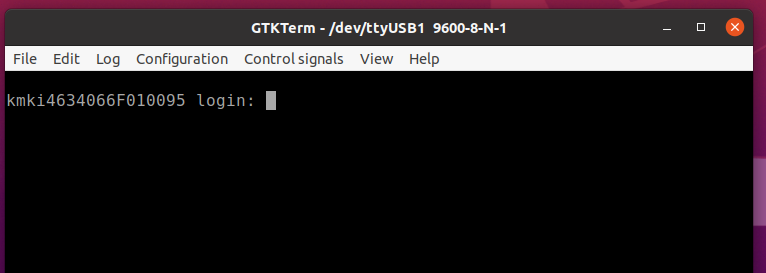
\includegraphics[width=\textwidth]{pic_08}
\end{center}
Введите логин root и пароль root.

\section{Подготовка наложенного дерева устройств}

Основная конфигурация целевой платы предполагает, что практически все выводы настроены для управления через блок GPIO. Для работы с I2C, необходимо ввести две правки: разрешить работу I2C контроллера и передать под его управления выводы, для коммуникации с внешним миром.  

Процессор на плате содержит три конролера I2С, однако воспользоваться возможно только одним, так как выводы вторых двух заняты контроллером карты памяти (sdhci), и при их назначении на I2C интерфейс, Linux не сможет загрузится.

\subsection{} Создадим рабочую папку в виртуальной машине для создания наложенного дерева устройств и перейдём в неё 
\begin{lstlisting}[style=bash]
# mkdir -p $BAGET/lab_06/devtree
# cd $BAGET/lab_06/devtree 
\end{lstlisting}

\subsection{}Создадим новый файл
\begin{lstlisting}[style=bash]
# kate of_i2c2.dts
\end{lstlisting}
и запишем в него следующий текст
\begin{lstlisting}[style=stdout]
/dts-v1/;
/plugin/;
/ {
	fragment@0 {
		target-path = "/gpio@1b400380";
		__overlay__ {
			
			i2c2_pins {
				phandle = <0x01>;
				i2c2_scl {
					function = "i2c2_scl";
					groups = "i2c2_scl";
				};
				i2c2_sca {
					function = "i2c2_sca";
					groups = "i2c2_sca";
				};
			};
		};
	};
	
	
	fragment@1 { 
		target-path = "/i2c@1b400130"; 
		__overlay__ { 
			status = "okay"; 
			pinctrl-names = "default"; 
			pinctrl-0 = <0x01>; 
		}; 
	}; 
	
	
	__local_fixups__ {
		fragment@1 {
			__overlay__ {
				pinctrl-0 = <0x00>;
			};
		};	
	};
};
\end{lstlisting}

Первый фрагмент, это дополнение к ноде описывающей банк выводов D. В этом дополнении создаём конфигурацию, для передачи управления частью выводов I2C контроллеру. Будьте внимательны, не любой вывод может быть передан I2C контроллеру. 

Следующий фрагмент правок, касается дополнения к описанию i2c контроллера. Первое, это его активация, записью в параметр status значения okay. Так же, мы вводим два дополнительных параметра, один хранит в себе название конфигурации выводов, второй — для указания идентификатора конфигурации, обратите внимание, что значение у него совпадает (и это важно) со значением phandle у описания выводов из первого фрагмента.

Последняя строка гарантирует, что после применения этого дополнения, значение параметра pinctrl-0 будет соответствовать значению phandle нашей группы i2cs\_pins. Дело в том, что значение phandle из первого фрагмента, будет  актуализировано, для разрешения коллизий (так как в исходном device-tree уже есть нода, с таким значением phandle), и последняя строка в нашем описании исправлений поясняет системе, что после разрешения коллизии, необходимо обновить значение указанного параметра (значение 0 зарезервировано, и в данном контексте означает ссылку на значение параметра phandle).  

Узнать, какой банк выводов, и какие выводы могут быть использованы с тем или иным интерфейсом, какие значения phandle уже использованы, и просто для любопытства можно одним из двух способов:

\begin{enumerate}
	\item Из самой системы, изучив подкаталоги gpio, в каталоге /proc/device-tree/ (рекомендуется для считывания значение того или иного параметра использовать команду cat). 
	
	\item Преобразовав бинарный файл device-tree системы в текстовый вид 
	\begin{lstlisting}[style=bash]
		# dtc -@ -O -dts -o  /tmp/root.dts \
		$BAGET/support/barebox/k5500vk018_rbm.dts
		# kate /tmp/root.dts
	\end{lstlisting}
\end{enumerate}

Посмотрите на ноды, описывающие банки GPIO выводов. Так же обратите внимание, на объявление конфигураций выводов для sdhci контроллера, особенно, как эта конфигурация разбита, между двумя банками выводов, на значение параметра phandle каждой группы. Сравните значение параметров phandle конфигурационных груп, и значения перечисленные в параметре pinctrl-0 у ноды для контроллера  sdhci. (не стесняйтесь использовать поиск по файлу).

\subsection{}Сохраните изменения Ctrl+S и закройте редактор Ctrl+Q 

\subsection{}Скомпилируем и отправим файл на плату
\begin{lstlisting}[style=bash]
# dtc -@ -O dtb -o ./of_i2c2.dtb ./of_i2c2.dts
# scp ./of_i2c2.dtb netuser@192.168.100.200:/home/netuser/
\end{lstlisting}

\subsection{}Перейдите в терминал платы, и переместите файл в папку barebox
\begin{lstlisting}[style=bash]
$ mv /home/netuser/of_i2c2.dtb /barebox/
\end{lstlisting}

\subsection{}Внесити правкив вайл barebox.sh
\begin{lstlisting}[style=bash]
$ nano /barebox/barebox.sh
\end{lstlisting}
Впишите после строки DTB=k5500vk018\_rbm.dtb следующую строчку
\begin{lstlisting}[style=stdout]
fdt_apply -i $DTB -l of_i2c2.dtb -o /dtb && DTB=/dtb
\end{lstlisting}
Сохраним изменения и выйдем из редактора (Ctrl+S, Ctrl+X).

\subsection{}Перезагрузите плату командой reboot.

\subsection{}После перезагрузки входим в систему (root/root). И выполняем команду
\begin{lstlisting}[style=bash]
$ ls /dev/i2c*
\end{lstlisting} 

В выдачи должен присутствовать файл i2c-0. Если его нет, выполните команду dmesg на целевой платформе, и изучите лог загрузки, на предмет ошибок инициализации I2C контроллера, при их остутствии, перезагрузите плату, и изучите лог работы загрузчика, на пример ошибок в наложеном дереве устройств.

\section{Работа с I2C из user-space}

\subsection{}Подключите модуль HW-290 к плате, как показано на рисунке 
\begin{center}
	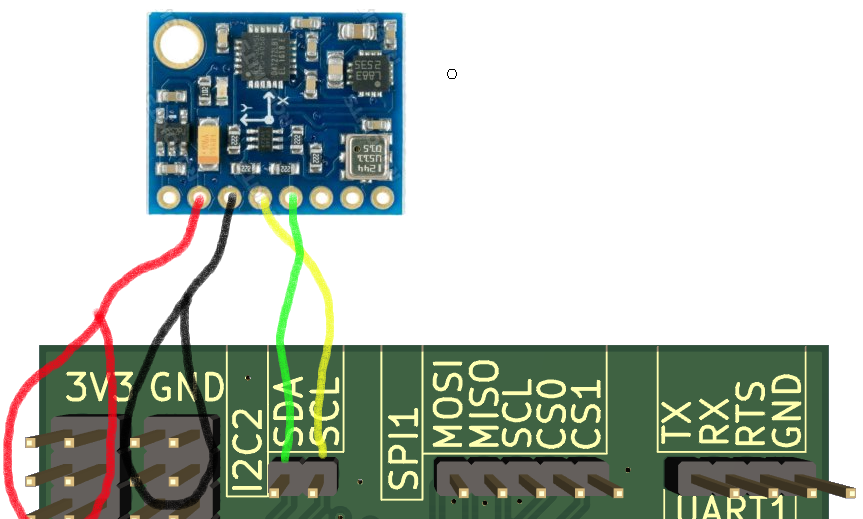
\includegraphics[width=0.7\textwidth]{pic_21}
\end{center}

\subsection{}Просканируем доступные к взаимодействию I2C устройства, а так же узнаем их адреса. Для этого воспользуемся командой i2cdetect
\begin{lstlisting}[style=bash]
# i2cdetect -y 0
\end{lstlisting}
где 0 это индекс i2c адаптера, вспомните что выдала команда ls /dev/i2c*.

\begin{center}
	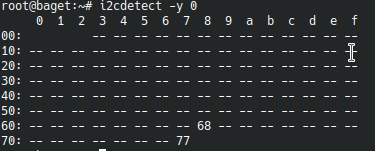
\includegraphics[width=0.7\textwidth]{pic_22}
\end{center}

Могут возникнуть ошибки при сканировании, убедитесь, что к выводам I2C контроллера подключены подтягивающие к питанию резисторы, и модуль подключен корректно.


\subsection{}Скопируем пример программы работающей с I2C и откроем её в редакторе vscode
\begin{lstlisting}[style=bash]
# cp -r $BAGET/support/i2c_app $BAGET/lab_06/app
# cd $BAGET/lab_06/app; code .
\end{lstlisting}

Проект состоит из нескольких файлов. Первый, это основной файл программы appi2c.c. Два других являются обёртками, для взаимодействия с I2C интерфейсом.

\subsection{}Скомпилируем приложение
\begin{lstlisting}[style=bash]
# make
\end{lstlisting}

\subsection{}И если ошибок не появилось, отправим программу на плату
\begin{lstlisting}[style=bash]
# scp $BAGET/lab_06/app/app \
netuser@192.168.100.200:/home/netuser
\end{lstlisting}

\subsection{}Запустим скопированное приложение на плате
\begin{lstlisting}[style=bash]
$ /home/netuser/app
\end{lstlisting}

Программа должна успешно подключиться к модулю, и выдавать в консоль данные с акселерометра.

\subsection{}Остановите работу программы нажав Ctrl+C

\subsection{} Выключите плату, для чего в начале введите команду
\begin{lstlisting}[style=bash]
	$ poweroff
\end{lstlisting}
дождитесь, как появиться надпись
\begin{lstlisting}[style=stdout]
	reboot: System halt
\end{lstlisting}
после чего отключите USB кабель от ПК или платы. 

\section{Задание для самостоятельной работы}

Допишите программу так, что бы она сообщала, о направлении перемещения в плоскости XY (вверх, вниз, налево, направо)

\subsubsection{*} Собрать модуль ядра, который будет обеспечивать коммуникацию через I2C интерфейс с акселерометром. Считывание данных об измеренном ускорении по осям через файл в папке /dev.